\section{RC5}
Im Folgenden sollen alle wichtigen Facts zu und über RC5 gegeben werden.

\subsection{Protokoll}
Hier die wichtigsten Facts 
\begin{itemize}
    \item Codelänge beträgt 24.889ms
    \item Pause zwischen Wiederholungen beträgt 88.889ms
    \item Code ist \emph{biphase}-coded\footnote{
        \emph{biphase-coded} kann frei als Flankengetriggert übersetzt
        werden. Siehe Codebeispiel im Bild \ref{pic:rc5_simple} }
    \item Code besteht aus 14-Bit Word
    \begin{itemize}
        \item 2 Start Bits
        \item 1 Toggle Bit
        \item 5 Systemadress-Bits
        \item 6 Kommando-Bits
    \end{itemize}
\end{itemize}

\begin{figure}[h!]
    \centering
    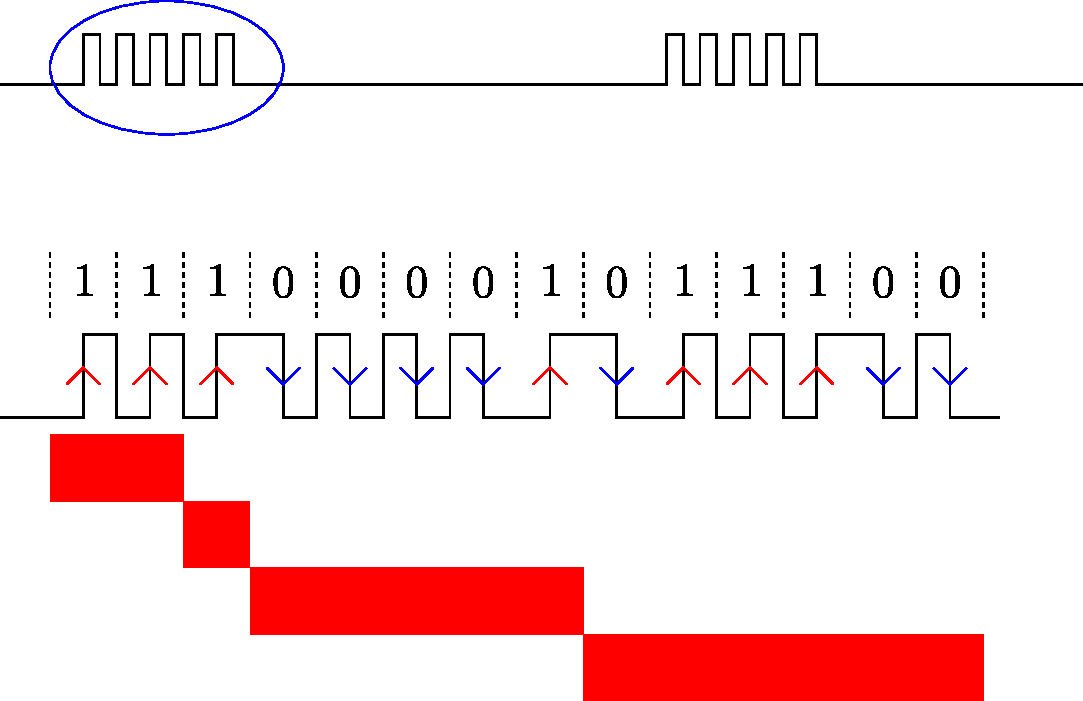
\includegraphics[width=0.8\textwidth]{rc5_simple.pdf}
    \label{pic:rc5_simple}
    \caption{RC5 Protokoll}
\end{figure}

\subsubsection{Start-Bits}
Das Startsignal besteht aus zwei Bits. Zuerst das eigentliche Start-Bit
und dann das sogenannte Field-Bit. Das Startbit ist immer logisch 1 und
stellt beim Empfänger die Verstärkung ein zum einlesen der Daten.
Das Field-Bit wird verwendet um dem Empfänger mitzuteilen, ob man den
unteren (0-63) oder oberen (64-127) Kommandobereich verwendet.
\subsubsection{Toggle-Bit}
Das Toggle- oder auch Steuer-Bit wird dazu verwendet permanentes (bzw. 
wiederholendes) senden von neuem Senden zu unterscheiden.
Dies ist nützlich um z.b. zu erkennen ob eine Taste dauerhaft gedrückt ist
bei der Fernbedienung etc.
\subsubsection{Systemadress-Bits}
Die 5 Systemadress-Bits erlauben es zwischen 32 verschiedenen Geräten
zu operieren.
\subsubsection{Kommando-Bits}
Die 6 Kommando-Bits bieten ein Set von 64 Befehlen an, mit welchem ein
Gerät (welches mit den 5 Systemadress-Bits spezifiziert wurde) angesteuert
werden kann.

\subsection{System-Adressen}

\begin{table}[h!]
    \footnotesize
    \centering
    \begin{tabular}{c l c l c l c l}
    Adresse & Gerät & Adresse & Gerät & Adresse & Gerät & Adresse & Gerät 
    \\
    \hline &&&&&&& \\
    00      & TV1       & 08 & Sat.-Rec 1   & 16 & Audio-PreAmp 1       & 24 & -                \\
    01      & TV2       & 09 & Camera       & 17 & Reciever/Tuner       & 25 & -                \\
    02      & Teletext  & 10 & Sat.-Rec 2   & 18 & Audio Tape Rec.      & 26 & CDR              \\
    03      & Video VD  & 11 & -            & 19 & Audio PreAmp 2$^*$   & 27 & -                \\
    04      & Video LV1 & 12 & Video-CD     & 20 & CD-Player            & 28 & -                \\
    05      & VCR1      & 13 & Camcorder    & 21 & Plattenspieler       & 29 & Beleuchtung 1    \\
    06      & VCR2      & 14 & -            & 22 & -                    & 30 & Beleuchtung 2    \\
    07      & exp.      & 15 & -            & 23 & DAT-T./MD-Rec.       & 31 & Telefon          \\
    \end{tabular}
    \caption{RC5 Systemadressen}
    \label{tab:rc5_systemadressen}
\end{table}
